% ----------------------------------------------------------
% Verification of Pipelined Processors
% ----------------------------------------------------------
\chapter{Verification of Pipelined Processors}
\label{chapther:pipeline}

This chapter presents a brief discussion on how IPC can be used to verify a pipelined processor. First, the concept of \textit{Pipelining} is reviewed with its main characteristics in Sec.~\ref{section:pipe-overview}. Then, an introduction on how to create an operational description of a pipelined processor along with a property example is presented in Sec.~\ref{section:ipc-pipe-processor}. Next, the notion of completeness for pipelined processors is discussed, including an introduction to the \SSQED{} approach, in Sec.~\ref{section:s2qed}. Finally, a discussion about the PDD method for Pipelined Processors is presented in Sec.~\ref{section:pdd-pipe-processor}.  

\section{Overview of Pipelined Processors}
\label{section:pipe-overview}

\textit{Pipelining} is a technique used to allow overlapping execution of instructions in a single core of a processor \cite{book-comp-org}. Instead of having instructions executing one after another in a sequential manner, the execution path for the instruction is divided into steps, called \textit{pipeline stages}. Thus, multiple instructions can overlap in time, each one executing in a different stage of the pipeline, Fig.~\ref{fig:pipe-example}.

\begin{figure}[htb!]
	\centering
	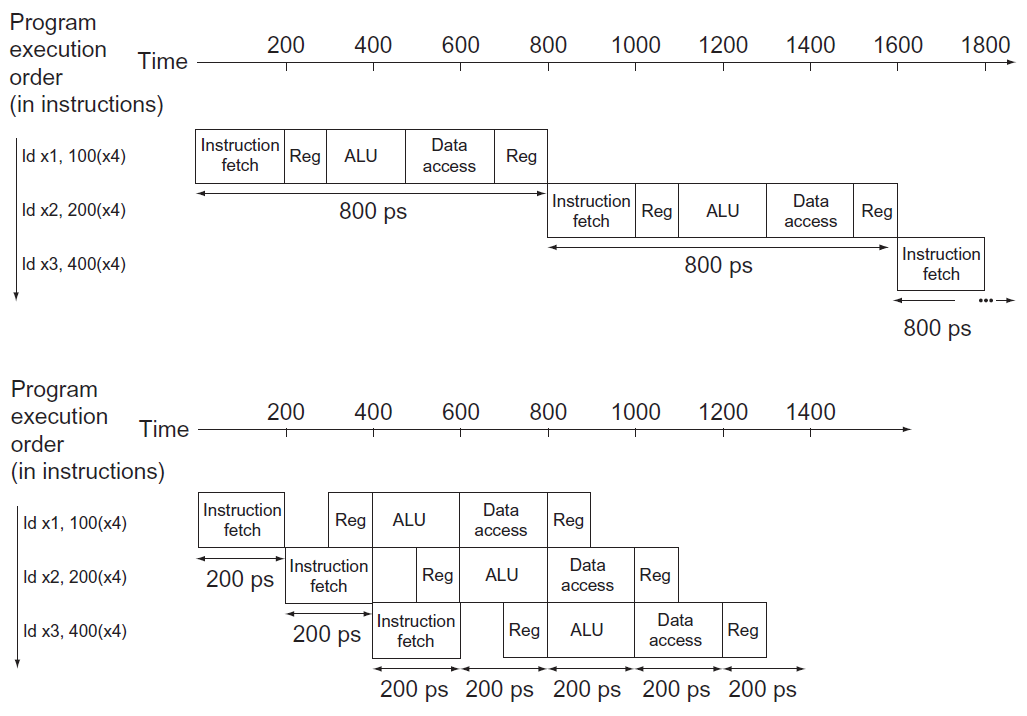
\includegraphics[width=0.85\textwidth]{images/pipeline-example.PNG}
	\caption{Illustration of the execution of instructions in a nonpipelined processor (top) versus pipelined execution (bottom). The \textit{ld} instruction loads data from the memory into a register in the processor register file. In this example, memory \textit{stalls} are not considered. (Reprinted from \cite{book-comp-org})}
	\label{fig:pipe-example}
\end{figure}

Since different types of instructions have very similar execution \textit{steps}, each step on the data path can be turned into a pipeline stage. For example, a common partition adopted in different pipelined processor implementations is: 

\begin{itemize}
\item Instruction Fetching (\textit{IF}): fetches a new instruction from memory to feed the pipeline;
\item Instruction Decoding (\textit{ID}): decodes instruction \textit{opcodes} and reads its operands from the register file;
\item Execution (\textit{EX}): executes the instruction operation. Usually associated with ALU operations;
\item Data Access (\textit{MEM}): performs \textit{read} and \textit{write} operations with data memory;
\item Write back (\textit{WB}): writes back the operations results or loaded data from data memory.
\end{itemize}

Certainly, each processor can have its own pipeline implementation, but they usually constitute some variation of the five presented stages.

One main advantage of pipelining is increasing the instruction \textit{throughput}, the amount of processed data per time unit. This advantage is illustrated in Fig.~\ref{fig:pipe-example}. In this example, a single \textit{load} instruction takes 800\,ps in a nonpipelined processor. Considering a pipelined processor with the five aforementioned stages, and with each stage taking 200\,ps, the three \textit{load} instructions execute in 1400\,ps, in contrast to the 2400\,ps needed for the nonpipelined processor. In this example, of course, possible \textit{stalls} caused by waiting for data memory are not considered for simplicity reasons. 
\TLSAY{If the frequency remains the same non-pipelined would be better because we get 1 instruction / cycle where as in pipelined we get (1/number of stages) instructions / cycle. 
Right? }
\section{Property Checking for Pipelined Processors}
\label{section:ipc-pipe-processor}

In order to verify the design by property checking, the processor behaviour has to be described in term of operations, see Sec.~\ref{section:formal-verification}. There are many ways to achieve that, but one simple and intuitive way is to consider an operation as the complete execution of an instruction through all the pipeline stages. This operational description is more intuitive because the behaviour of each instruction is already specified in the \textit{Instruction Set Architecture}~(ISA) of the corresponding implemented processor, and it is simpler than specifically describing different combinations of instructions at different pipeline stages at time.

Since every operation starts and ends at an \textit{important state}, a common pipeline stage can be chosen as the initial and final state. As an example, one may consider the \textit{IF} stage as the \textit{important state} and that every operation starts being fetched and ends when the next instruction is fetched. In practice, when the \textit{Instruction Under Verification}~(IUV) moves from \textit{IF} to \textit{ID}, the next instruction is already fetched.

A complete set of properties needs to prove all \textit{outputs} and \textit{visible registers} at all times, see Sec.~\ref{subsection:notion-completeness}, according to determination requirements. For this operational description of pipelined processor, one property will prove \textit{outputs} and \textit{visible registers} corresponding to each pipeline stage. Consider the property in Fig.~\ref{fig:ex-add-ppt}. It depicts an example of a property proving the \textit{ADD} instruction in a 4-stages pipeline processor. The \textit{Program Counter} (PC) is proven only at the \textit{ID} stage, $t\_ID$. This does not compromise the completeness if there is always a property proving PC at all times. For example, at $t\_IF$ the previous instruction is at the \textit{ID} stage and proves the PC, and at $t\_EX$ is the instruction succeeding the IUV which is at the \textit{ID} stage proving the PC.

\begin{figure}[htb!]
    \begin{lstlisting}
    property ADD;
    assume:
        //conceptual state
        at t_IF: conceptual_state;
        at t_IF: empty_pipeline;
    
        //Trigger
        at t_IF: instr_type(fetched_instr) == ADD;
    prove:
        at t_ID: conceptual_state;
        at t_ID: PC == PC_at_t_IF + 4;
    
        at t_EX: ALU_oper_a == getOperA(fetched_instr);
        at t_EX: ALU_oper_b == getOperB(fetched_instr);
        at t_EX: ALU_result == ALU_oper_a + ALU_oper_b;
        
        at t_WB: regile_wb == ALU_result;
    
        at t_end: REGFILE(reg_dest) == ALU_result;
    end property;\end{lstlisting}
    \caption{Example of a property describing the execution of the \textit{ADD} instruction in a pipelined processor.}
    \label{fig:ex-add-ppt}
\end{figure}

In the example property for an \textit{ADD} instruction in Fig.~\ref{fig:ex-add-ppt}, the processor \TLSAY{The processor is now a computational model. We select all states that relate to the conceptual state} is in a state called \textit{conceptual\_state} at $t\_IF$, line 4 \TLSAY{dont do this , line~x ... rather do ... Line 4, shows ... In line 4 xyz ... or (see line~x)}. This conceptual state corresponds to a state where the processor is ready to fetch a new instruction. When the IUV is at the \textit{ID} stage, the processor should be again at the conceptual state and ready to fetch a new instruction, line 10. Back to the assumptions, the property states that the fetched instruction is of type \textit{ADD}. In the commitments, the visible register PC is proved to be incremented by four at $t\_ID$. At $t\_EX$, the property proves that the ALU receives the right operands and computes the right result. At $t\_WB$, the right result is sent back to the register file. Finally, at $t\_end$, the destination register in the register file holds the right computed result.

A property set that covers the \textit{reset} behaviour and has one property for every possible instruction in the ISA will pass the completeness tests for successor, determination, and reset (see Sec.~\ref{subsection:notion-completeness}). However, the case-split test will not hold. This is because the properties referred so far assume that the IUV execution is not influenced by any other instruction in the pipeline. Line 5 in the listing of Fig.~\ref{fig:ex-add-ppt} assumes that the pipeline is empty when the IUV is fetched. Obviously, in practice this will hardly be the case. In order to overcome this problem, an approach called \SSQED{} \cite{paper-symbolic} can be employed. The next section presents an overview of this approach.

\section{Completeness with \SSQED{}}
\label{section:s2qed}

\SSQED{} \cite{paper-symbolic} is a verification approach based on a bounded model with symbolic initial state. It offers a proof that the execution of each instruction is independent of its \textit{program context}. In other words, each instruction executes independently of other instructions currently in the pipeline. 

Errors in hardware design are often called “\textit{bugs}” or “\textit{logic bugs}”. In \cite{paper-gapfree}, these errors are defined as a deviation of the implementation’s behaviour from the specification. Also in \cite{paper-gapfree}, two categories of logic bugs are presented:

\begin{enumerate}
\item Single-instruction bug: it is defined when the \textit{opcode} and the operands of the IUV causes an error in all program contexts, i.e. independently of all previously executed instructions.
\item Multiple-instruction bug: it is defined when it is not a single-instruction bug and there exists an instruction \textit{opcode}, a set of operands and a program context such that the execution of the IUV leads to an error.
\end{enumerate}

The property set presented so far, composed with properties like the one in Fig.~\ref{fig:ex-add-ppt}, is able to identify single-instruction bugs since they are independent of the program context. Therefore, the \textit{empty\_pipeline} assumption will not interfere on finding these types of errors. On the other hand, this assumption will mask multiple-instruction bugs as they require specific instruction sequence scenarios in order to occur.

In order to exemplify a multiple-instruction bug, consider a \textit{read-after-write} hazard. This hazard happens, for example, when an instruction \textit{reads} a register that is written by its immediate previous instruction. In this case, considering the same 4-stages pipeline, the register value is read before the "write to the register file" operation is complete by the previous instruction. To avoid an error, pipelined processors implement a mechanism called \textit{forwarding}. This mechanism forwards the value that is going to be written in the register file to previous pipeline stages, so it can be used by the following instruction if needed. A bug in the forwarding structure is considered a multiple-instruction bug as it does not depend only on the IUV, but in previous instruction fed into the pipeline. 

The \SSQED{} approach covers multiple-instruction bugs by assigning one same instruction, at an arbitrary time point, to execute in two \textit{identical} and \textit{independent} instances of the processor under verification. The computational model of the \SSQED{} approach is depicted in Fig.~\ref{fig:s2qed-model}.

\begin{figure}[htb!]
	\centering
	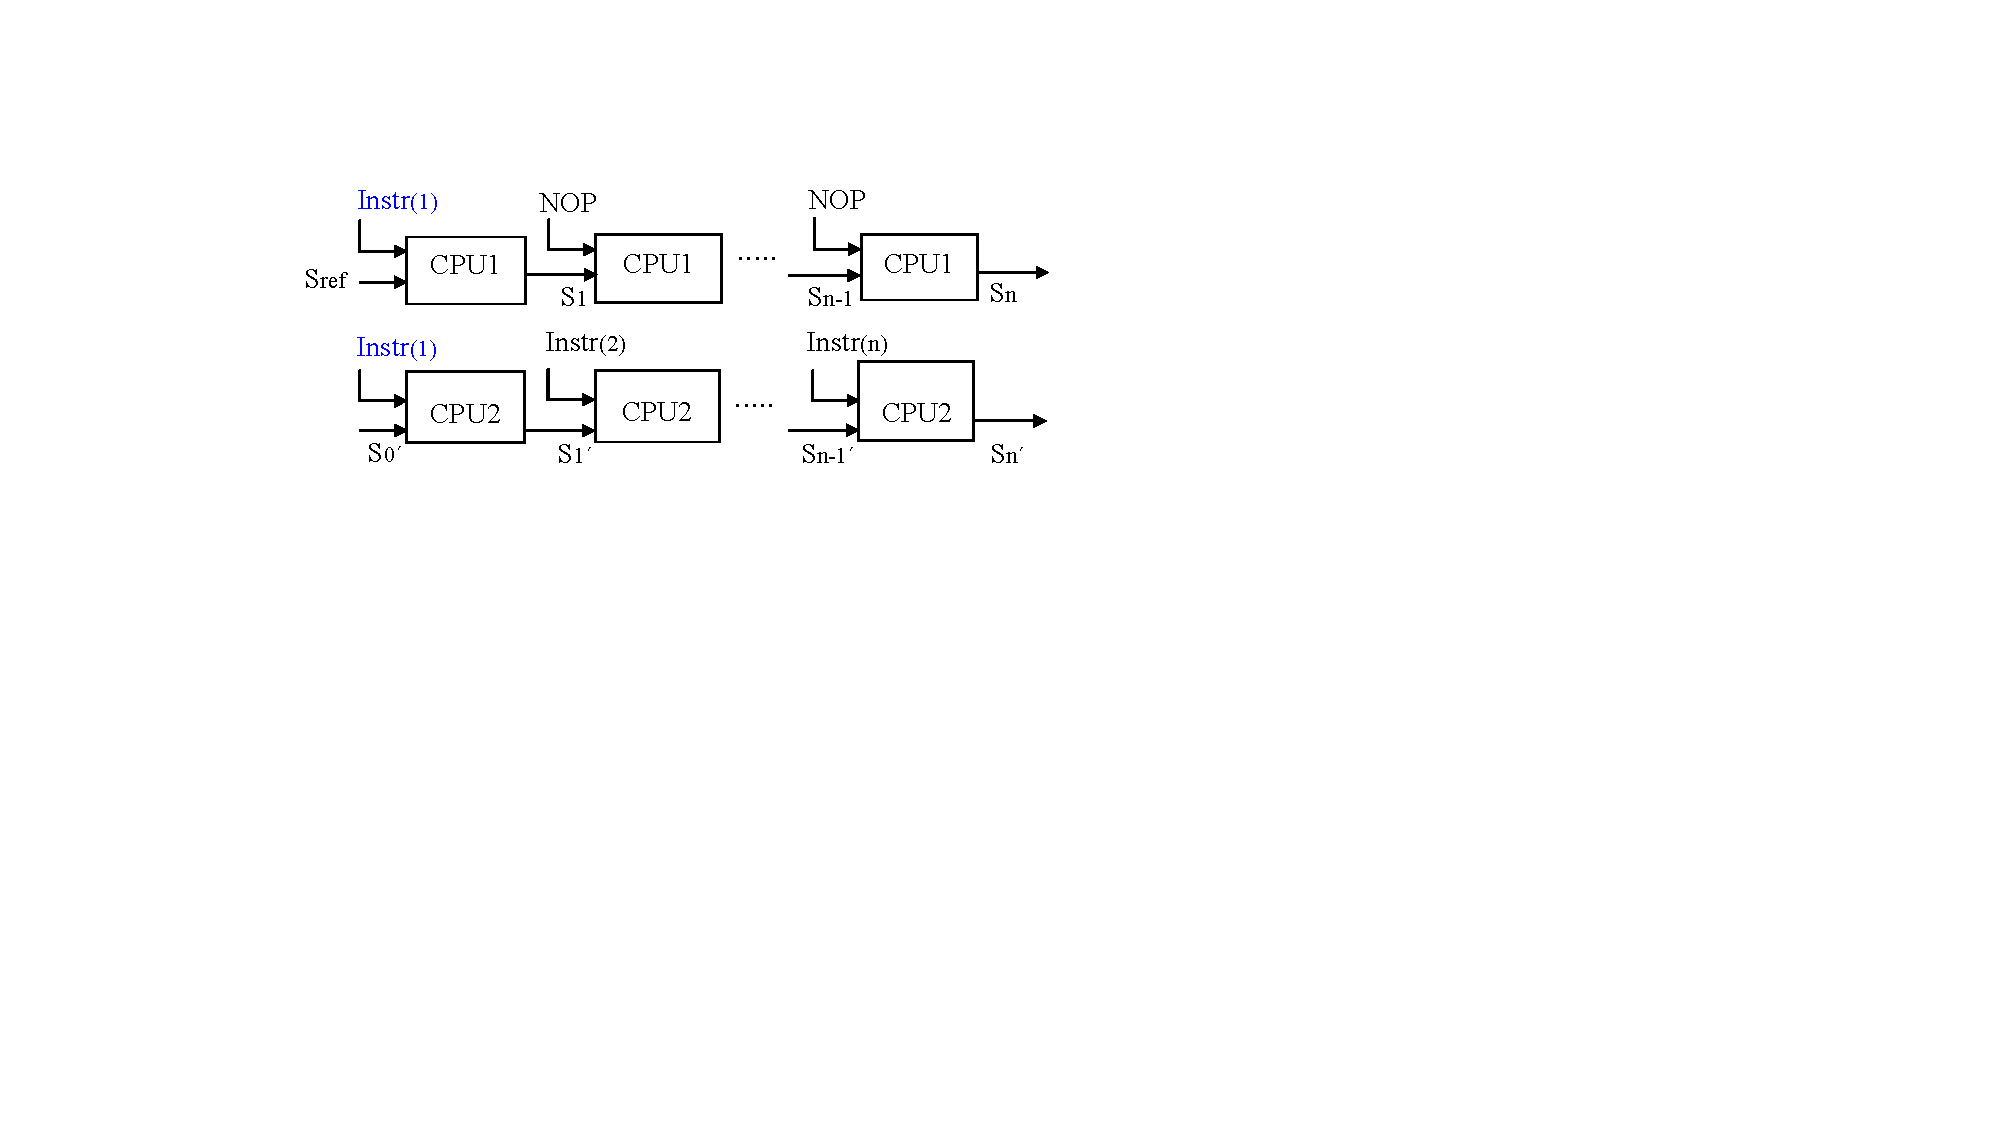
\includegraphics[width=0.7\textwidth]{images/s2qed_model.pdf}
	\caption{\SSQED{} computational model. Both constrained and unconstrained instances, \textit{CPU1} and \textit{CPU2} respectively, execute the same IUV. (Reprinted from \cite{paper-gapfree})}
	\label{fig:s2qed-model}
\end{figure}

The first CPU instance, in the same manner as the CPU model considered so far, is constrained to execute the IUV in an empty pipeline. The second CPU instance is unconstrained to execute an arbitrary sequence of instructions. The only restrictions for the second CPU instance are that it fetches the same instruction as the first instance at time $t$, and they both are consistent. This required consistency, named \textit{QED-consistency}, is defined in \cite{paper-gapfree} as follows:

\begin{quote}
     \textit{"In the \SSQED{} computational model, the two CPU instances are QED-consistent at a time $t$, if the corresponding architectural state elements of both instances at time point $t$ hold the same values."}
\end{quote}

For this \SSQED{} computational model, the SAT-Solving tool will compare the execution of the IUV in the constrained empty pipeline of the first CPU instance with all the scenarios for the unconstrained execution of the IUV in the second CPU instance, including the context where the multiple-instruction bugs appear and propagate. The listing on Fig.~\ref{fig:ex-s2qed-add-ppt} shows an example of an \SSQED{} property for an \textit{ADD} instruction.

\begin{figure}[htb!]
    \begin{lstlisting}
    property S2QED_ADD;
    assume:
        // constraints on CPU1
        at t_IF: cpu1_conceptual_state;
        at t_IF: cpu1_empty_pipeline;
        during [t_IF+1, t_WB]: instr_type(cpu1_fetched_instr) == NOP;
    
        // same IUV
        at t_IF: cpu1_fetched_instr == cpu2_fetched_instr;
        at t_IF: instr_type(cpu1_fetched_instr) == ADD;
    
        // QED consistent registers
        at t_WB: qed_consistency_registers();
    
    prove:
        at t_end: qed_consistency_registers();
        end property;\end{lstlisting}
    \caption{Example of a \SSQED{} property describing an \textit{ADD} instruction as the IUV.}
    \label{fig:ex-s2qed-add-ppt}
\end{figure}

Lines 4 and 5 of the property in Fig.~\ref{fig:ex-s2qed-add-ppt} constrain the \textit{CPU1} instance to be on the conceptual state and have an empty pipeline. The assumption in line 6 constrains the \textit{CPU1} to fetch only \textit{NOP} instructions after fetching the IUV. This assumption is not crucial to prove the model, however, it reduces unnecessary complexity for the SAT-solving tool. The assumptions on lines 9 and 10 will bind the IUV in both CPU instances to be the same and of type \textit{ADD}. Finally, the last assumption on line 13 comprises the QED-consistency, which is also proven on the commitment on line 16.

The macro function \textit{qed\_consistency\_registers()} expresses the Boolean function shown in Eq.~\ref{eq:consistency-register}. It characterizes the QED-consistency register state for a processor with $N$ registers on its register file.

\begin{equation}
    qed\_consistency\_registers := \,\, \bigwedge_{i = 0}^{N-1} \left(R^i_{cpu1} = R^i_{cpu2}\right)
    \label{eq:consistency-register}
\end{equation}

The consistency between the two CPU instances is the key for accomplishing completeness solving the case-split test. The \SSQED{} computational model guarantees a consistent result of every operation between both instances. Therefore, proving the case-split test for one of the instances is sufficient.

The case-split test is easy to satisfy for a set of \SSQED{} properties, since every possible instruction sequence is implicitly considered on the \textit{CPU2} instance. For a formalism on how the case-split test is proven on a \SSQED{} property set, the reader may refer to \cite{paper-gapfree}.

\section{PDD for Pipelined Processors}
\label{section:pdd-pipe-processor}

The Property-Driven Design approach, see Sec.~\ref{section:PDD}, generates operational properties from an ESL design described in SystemC-PPA in order to prove that the later implemented RTL design is sound with respect to the ESL. The SystemC-PPA description is a sequential model from which the extracted operations represent transitions between important states. 

A pipelined processor will have its operations overlapping in time, for each operation represents an instruction executing throughout the pipeline stages. Consequently, while the ESL model describes the behaviour of instructions of a program executing sequentially one after another in the processor (see the execution on top of Fig.~\ref{fig:pipe-example}) the RTL implements the pipeline where an instruction starts executing before the previous one is completed. This concurrent behaviour is shown on the bottom of Fig.~\ref{fig:pipe-example}.

If the ESL model does not describe the concurrent execution of operations, the generated PPA will not match the pipeline implemented in the RTL. In practice, the \textit{DeSCAM} tool (see Sec.~\ref{subsection:PDD-flow}), that generates the properties, derives the important states from communication transactions in the DUV, so the operations represent the data manipulation between communication. 

Let us consider the 4-stage pipeline processor defined in this chapter with two communicating interfaces. One memory interface to fetch instructions and the other for communication with the data memory. Fig.~\ref{fig:ppa-seq} shows the PPA extracted from the sequential SystemC-PPA description of the processor. 

\begin{figure}[htb!]
	\centering
	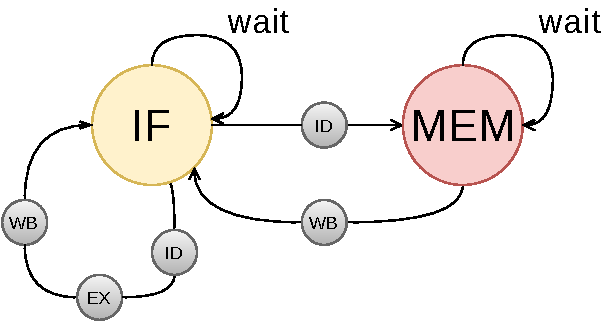
\includegraphics[width=0.6\textwidth]{images/PPA_old.pdf}
	\caption{PPA for a sequential SystemC-PPA processor description.}
	\label{fig:ppa-seq}
\end{figure}

The bigger circles in the PPA of Fig.~\ref{fig:ppa-seq} represent important states where there is some transaction with a communication port, while the smaller circles represents unimportant states. There are two important states, the \textit{IF} state that communicates with the instruction memory, and the \textit{MEM} state that communicates with the data memory.

The listing of Fig.~\ref{fig:ex-pdd-add-ppt} shows an example of a property generated for an \textit{ADD} instruction from a sequential ESL. The time $t$ corresponds to the fetching time, and the time $t\_end$ to the time point after the write back, $t+4$. The property is triggered when the CPU is ready to fetch, \textit{conceptual\_state}, and a new instruction of type \textit{ADD} is fetched. At $t\_end$, after the \textit{ADD} instruction is completely executed, the commitments prove that the right result is written to the right destination register.

\begin{figure}[htb!]
    \begin{lstlisting}
    property PDD_ADD;
    assume:
        at t: conceptual_state;
        at t: instr_type(fetched_instr) == ADD;
    prove:
        at t_end: conceptual_state;
        at t_end: PC == PC_at_t + 4;
        at t_end: REGFILE(reg_dest) == ADD_result;
        
        //intruction memory interface
        during [t+1, t_end-1]: instr_req_out_notify == false;
        at t_end: instr_req_out_notify == true;
        
        //data memory inteeface
        during [t+1, t_end]: data_req_out_notify == false;
    end property;\end{lstlisting}
    \caption{Example of a property for the \textit{ADD} instruction generated from a sequential PPA.}
    \label{fig:ex-pdd-add-ppt}
\end{figure}

It is important to notice that the request signal to fetch a new instruction is only asserted at the time point $t\_end$, being set to false during the whole instruction execution time. Similarly, the request signal for the data memory is de-asserted all the time since the \textit{ADD} instruction does not communicate with the data memory at any time. As a result, a set with $n$ properties corresponding to the $n$ instructions of the processor ISA will not hold for the RTL design. One problem can be easily spotted in this example. Consider the operation property for a \textit{LOAD} instruction, while the \textit{ADD} property tries to prove that the \textit{data\_req\_out} signal is always false, the \textit{LOAD} instruction tries to prove that the same signal is set to true during the memory phase.

Two approaches could be considered in order to apply the PDD flow for the design of a pipelined processor. First, the designer can redesign the ELS description so that it reflects the pipeline concurrent RTL behaviour. In this case, the ESL abstraction is lost because RTL implementation details are replicated at the ESL model. The second alternative is refining the pipeline within the macros for the generated instructions. Once again, the designer would have to replicate part of the RTL implementation, this time during the refinement of the macros. 

For both approaches, additional effort by the designer is required, which mitigates the goal of applying the PDD method, that is to accelerate the design process. Chapter~\ref{chapter:algorithm} presents how the PDD approach can be extended for pipelined processors by introducing small changes at the SystemC-PPA, and proposes an algorithm that can be used to convert the generated \textit{DeSCAM} properties into a property set that matches the pipeline concurrent behaviour. 

